\chapter{Chip Design and Characterization Results}

As discussed above, current approaches are either using relatively large electrodes, or have only used microelectrodes that were fabricated without specific regard for shape, size, distance and configuration. Thus, there is a need to identify the relationships among those characteristics and their impact on signal strength. This chapter describes the design goals of the chip, formulates hypothesis about its design, tests them, and draws some conclusions about the importance of shape, size, distance, and configuration. Tests are done with norepinephrine (NE) instead of NO because NO has a short lifespan, and NE performs similarly.

Previous work in this field is insufficient for our needs. We expect signals in the picoamp range on the microsecond timescale, and thus require circuitry able to amplify and measure quickly \cite{mosharok2005aee}. Other work has not addressed timing requirements \cite{zhang2005eam, steffan2007scp}, assumes slow concentration change times on the order of seconds \cite{murari2005ipn}, or uses oversampling (which is slow) to detect low concentrations \cite{murari2005ipn, stanacevic2007vpa}.

Due to the above limitations, a chip was designed that was able to meet the requirements, and test hypotheses, for integrated biosensing \cite{karegar2007ema}. The process used to achieve these goals was CMOS, the standard process used in microchip fabrication. Our process was able to produce feature definition at the 0.6 $\mu \mathrm{m}$ size. The electrodes are platinum on a glass substrate. There are 21 sensor sites, arranged in a $5 \times 5$ grid, with varying configurations and distances between electrodes, making each site unique (Figure \ref{biosensorchip-sensors}). Sensor sites are $500 \mu \mathrm{m}$ (center-to-center) apart. The size of the chip is $9 \mathrm{mm} \times 9 \mathrm{mm}$, with bonding pads on the exterior at $160 \mathrm{mm} \times 160 \mathrm{mm}$ each (Figure \ref{biosensorchip}).

\begin{figure}
	\centering
	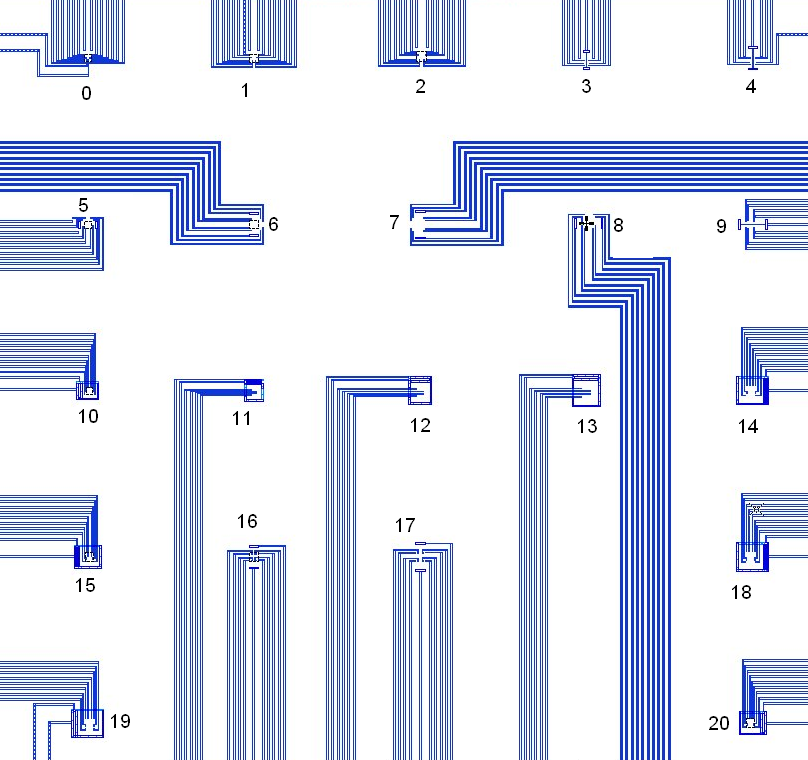
\includegraphics[width=0.8\linewidth]{figures/biosensorchip-sensors.png}
	\caption[Sensors layout of the chip]{Sensors layout of the chip with numbered sensors}
	\label{biosensorchip-sensors}
\end{figure}

\begin{figure}
	\centering
	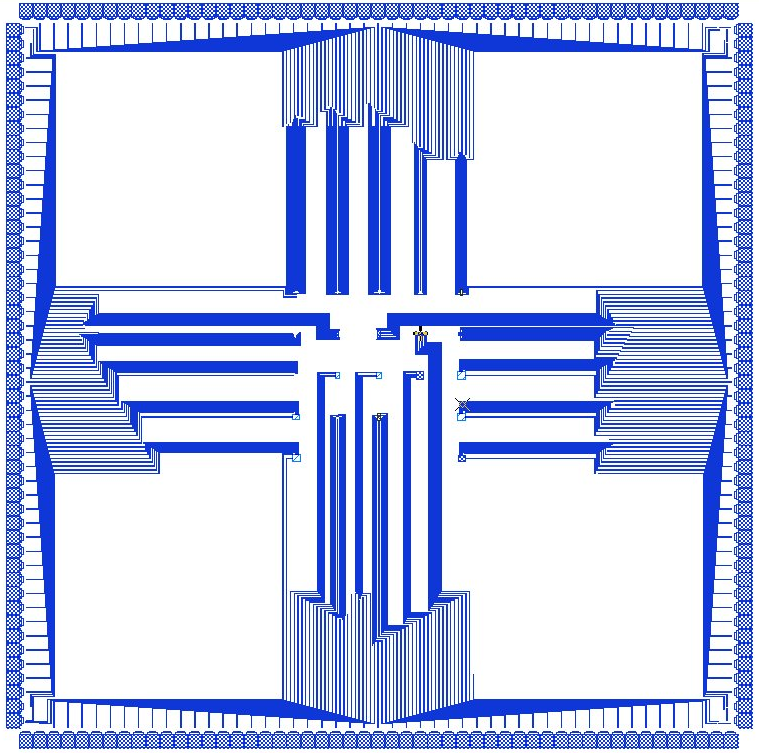
\includegraphics[width=0.5\linewidth]{figures/biosensorchip.png}
	\caption{Full layout of the chip}
	\label{biosensorchip}
\end{figure}

After the chip was fabricated, characterizations were done on each sensor site to determine the best shape, size, and organization of the electrodes. There are 21 sensor sites on the chip. Each sensor site has four working-electrode areas. Each area has either one or two working electrodes, depending on if it is a 3- or 4-electrode system, respectively. This chapter describes the chip, sensor sites, and electrode systems, and the experiments used to characterize them.

\section{Sensor Configurations}

There are 21 sensor sites on the chip. Each site uses one of four sensor-site configurations, and one of four working-electrode configurations.

\subsection{Working Electrodes}

Each site has 4 working-electrode areas. There are four configurations, which are either 3- or 4-electrode systems. Three electrode systems have one auxiliary electrode (AE), one reference electrode (RE), and one working electrode (WE). Four electrode systems have one AE, one RE, and two WEs. These two WEs can work in tandem (one as a generator, one a collector, with appropriate instruments), and are interdigitated \cite{frey2003dip}. The interdigitated design is done to increase interaction between the two electrodes. No tests here used such an instrument, but work on 4-electrode systems indicates larger output in those systems \cite{iwasaki1995emi}. To repeat, all 4-electrode systems were tested as if they were 3-electrode systems. The working-electrode configurations are (Table \ref{WE-size}):

\begin{description}
\item[3 electrode] where there is one WE, one RE, and one AE. WEs are numbered 1, 2, 3, 4, have areas ($\mu \mathrm{m}^2$) 1, 2.25, 4, 4, and perimeters ($\mu \mathrm{m}$) 4, 6, 8, 8, respectively.
\item[4 electrode, C shape] where there is one RE, one AE, and two WEs in the ``C'' shape (Figure \ref{4-C}). WEs are numbered 11, 12 for the first pair, 21, 22 for the second pair, 31 32 for the third pair, 41, 42 for the fourth pair. The first in each pair has area 10.885 $\mu \mathrm{m}^2$ and perimeter 24.700 $\mu \mathrm{m}$. The second in each pair has area 11.342 $\mu \mathrm{m}^2$ and perimeter 25.081 $\mu \mathrm{m}$.
\item[4 electrode, inverse C shape] where there is one RE, one AE, and two WEs in the ``inverse C'' shape (Figure \ref{4-I}). WEs are numbered 11, 12 for the first pair, 21, 22 for the second pair, 31 32 for the third pair, 41, 42 for the fourth pair. The first in each pair has area 14.267 $\mu \mathrm{m}^2$ and perimeter 30.793 $\mu \mathrm{m}$. The second in each pair has area 15.119 $\mu \mathrm{m}^2$ and perimeter 32.835 $\mu \mathrm{m}$.
\item[4 electrode, F shape] where there is one RE, one AE, and two WEs in the ``F'' shape (Figure \ref{4-F}). WEs are numbered 11, 12 for the first pair, 21, 22 for the second pair, 31 32 for the third pair, 41, 42 for the fourth pair. The first in each pair has area 21.771 $\mu \mathrm{m}^2$ and perimeter 46.636 $\mu \mathrm{m}$. The second in each pair has area 21.738 $\mu \mathrm{m}^2$ and perimeter 46.796 $\mu \mathrm{m}$.
\end{description}

\begin{figure}
	\centering
	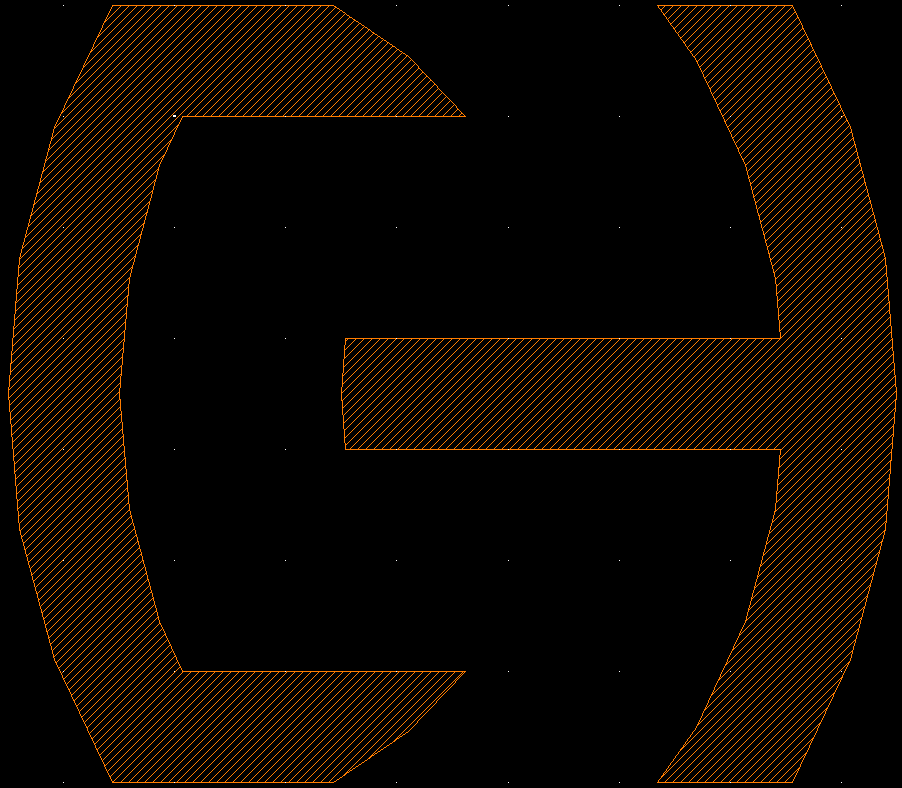
\includegraphics[width=0.1\linewidth]{figures/4-C.png}
	\caption{``C''-type working-electrode pair}
	\label{4-C}
\end{figure}

\begin{figure}
	\centering
	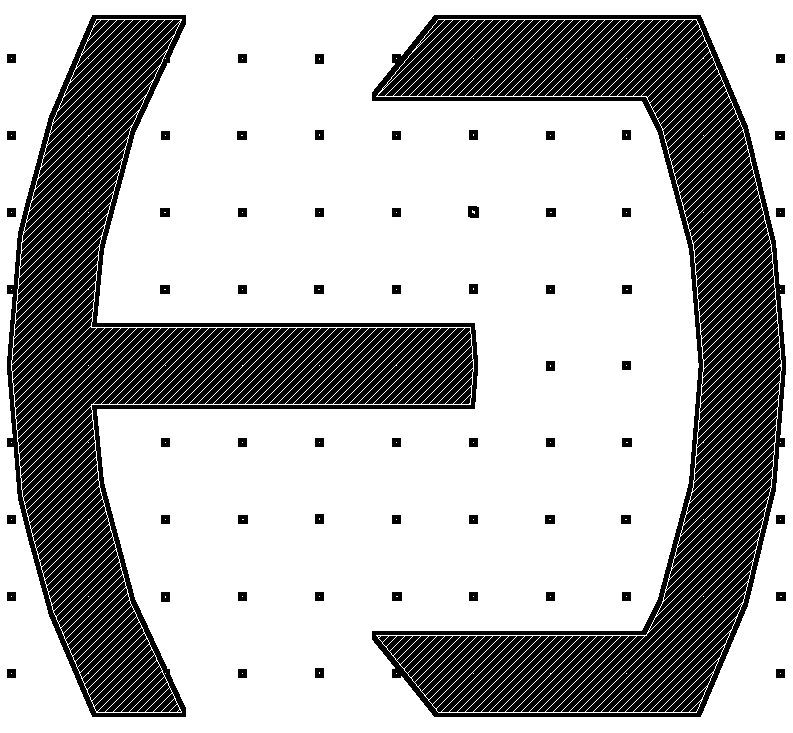
\includegraphics[width=0.1\linewidth]{figures/4-I.png}
	\caption{``Inverse C''-type working-electrode pair}
	\label{4-I}
\end{figure}

\begin{figure}
	\centering
	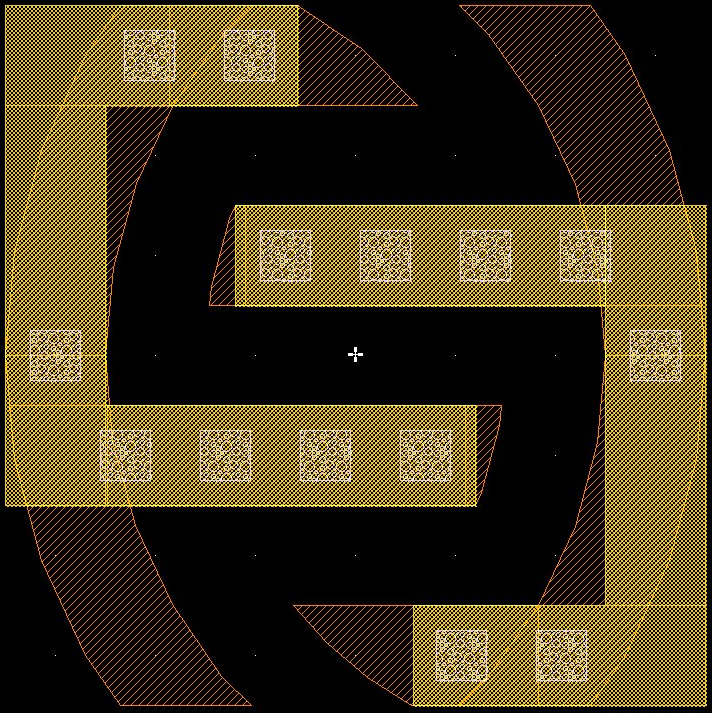
\includegraphics[width=0.1\linewidth]{figures/4-F.png}
	\caption{``F''-type working-electrode pair}
	\label{4-F}
\end{figure}

\begin{table}
	\begin{tabular}{l|l|l}
		\textbf{electrode system} & \textbf{areas} ($\mu \mathrm{m}^2$) & \textbf{perimeters} ($\mu \mathrm{m}$) \\
		\hline
		3 & 1, 2.25, 4, 4 & 4, 6, 8, 8 \\
		4, ``C'' & 10.885, 11.342 & 24.700, 25.081 \\
		4, ``inverse C'' & 14.267, 15.119 & 30.793, 32.835 \\
		4, ``F'' & 21.771, 21.738 & 46.636, 46.796
	\end{tabular}
	\caption[Working-electrode areas and perimeters]{Working-electrode areas and perimeters. The 3-electrode entry lists the different sizes that are in one sensor site. The 4-electrode entries list the areas of the first and second electrode in a pair, respectively.}
	\label{WE-size}
\end{table}

\subsection{Sites}

The sensor-site configurations are:

\begin{description}
\item[2 auxiliary] where there are four electrodes of the same size and spacing in a square with the WE at the bottom-left, RE at the top-right, and AEs at the top-left and bottom-right. The AEs are shorted together. This configuration is always in a 3-electrode system. This configuration is used as a control, as it is standard and simple.
\item[common reference, top \& bottom] where there are two large, common RE at the top and bottom of the sensor site. The WE and AE pairs have the same size (by pair), are square, and are placed between the common REs. The common REs are shorted together. This configuration is always in a 3-electrode system. In 3-electrode systems, there is no current into the RE. Thus, this configuration should perform equally to the above, 2-auxiliary configuration.
\item[common reference top, common auxiliary bottom] where there is a large, common RE at the top, and a large, common AE at the bottom. WE pairs are placed between. This configuration is always in a 4-electrode system. Since current does flow into the AE, this configuration should perform better than the above 2 configurations, since AE area is less of a limiting factor.
\item[common reference top, common auxiliary on 3 sides] where there is a large, common RE at the top, and a larger, common AE completely surrounding the RE, and surrounding the WEs on the top, bottom, and right sides. This configuration is used by both 3- and 4-electrode systems. Since the AE area here is much larger and closer to all WEs, this configuration should perform even betten than the previous. Since no current flows into the RE, it is believed that moving the AE closer to the WEs is a good design. Hence, the RE is surrounded by the AE, and the WEs are all closest to the AE.
\end{description}

\subsection{Sensors}

Of the sixteen possible sensor combinations, nine are used (Table \ref{sensor-config}):

\begin{description}

\item[Sensor 0] is a 3-electrode system, with 2 AEs (Figure \ref{s00}). WE areas have electrodes spaced at 3 $\mu \mathrm{m}$ for areas 1, 2, 4, and 2.5 $\mu \mathrm{m}$ for area 3. Pitch (center-to-center distance between WE areas) is $15 \mu \mathrm{m}$.
\item[Sensor 1] is the same as Sensor 0 (Figure \ref{s01}), but with a pitch of $20 \mu \mathrm{m}$.

\begin{figure}
	\begin{minipage}{0.5\linewidth}
		\centering
		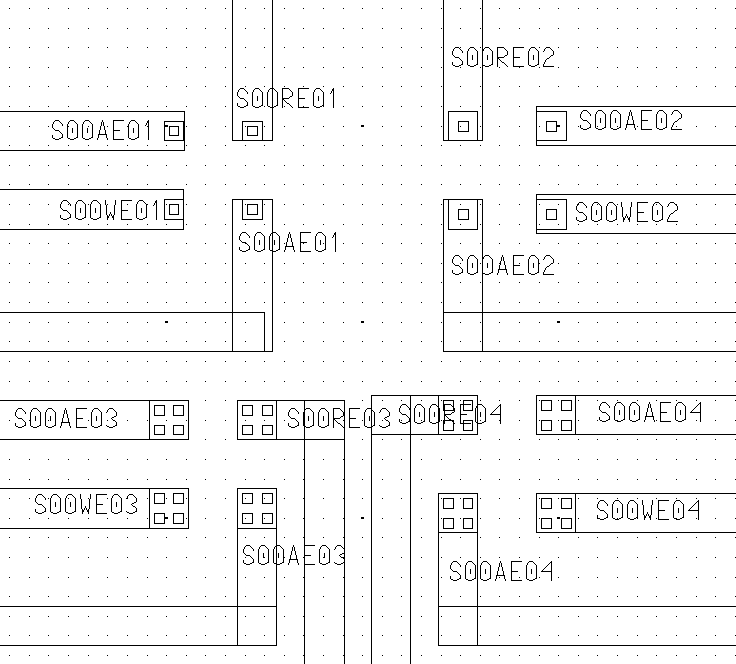
\includegraphics[width=0.6\linewidth]{figures/s00.png}
		\caption{Sensor 0}
		\label{s00}
	\end{minipage}
	\begin{minipage}{0.5\linewidth}
		\centering
		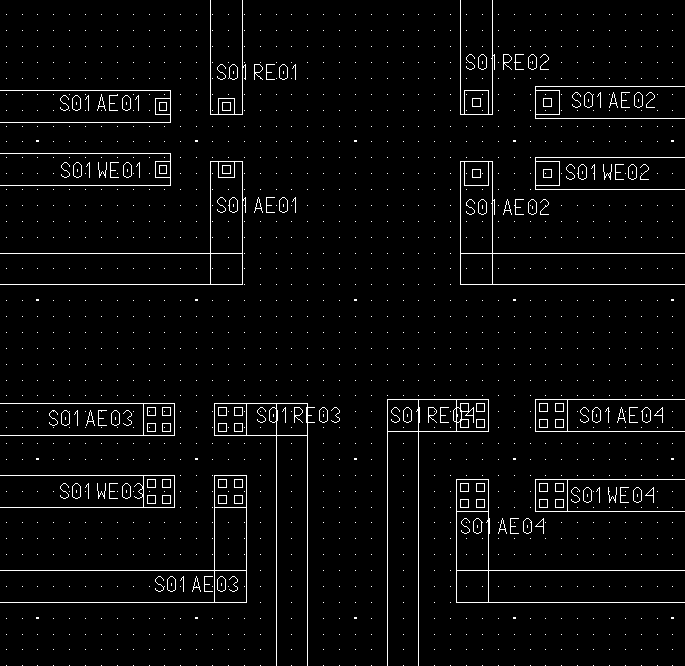
\includegraphics[width=0.6\linewidth]{figures/s01.png}
		\caption{Sensor 1}
		\label{s01}
	\end{minipage}
\end{figure}

\item[Sensor 2] is the same as Sensor 0 (Figure \ref{s02}), but with a pitch of $25 \mu \mathrm{m}$..
\item[Sensor 3] is a 3-electrode system, common RE at top and bottom (Figure \ref{s03}). WE areas have electrodes spaced at 3 $\mu \mathrm{m}$ for areas 1, 2, 4, and 2.5 $\mu \mathrm{m}$ for area 3. Pitch is $15 \mu \mathrm{m}$.

\begin{figure}
	\begin{minipage}{0.5\linewidth}
		\centering
		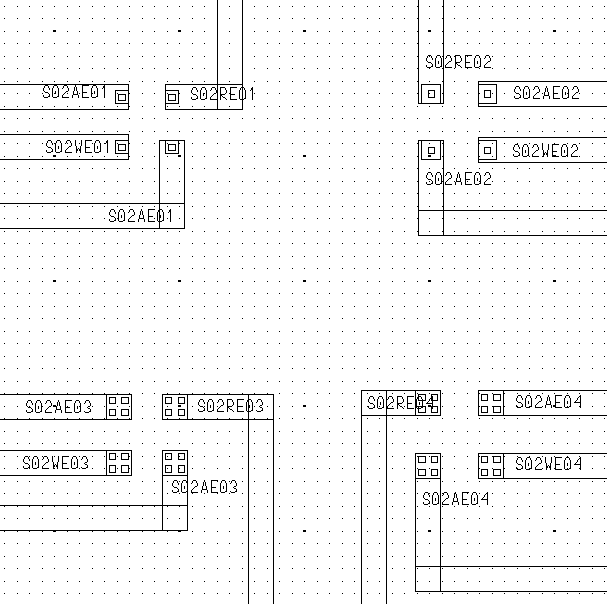
\includegraphics[width=0.6\linewidth]{figures/s02.png}
		\caption{Sensor 2}
		\label{s02}
	\end{minipage}
	\begin{minipage}{0.5\linewidth}
		\centering
		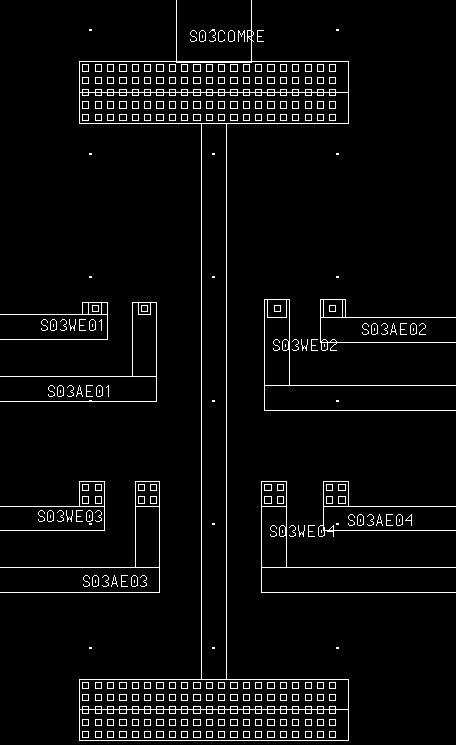
\includegraphics[width=0.6\linewidth]{figures/s03.png}
		\caption{Sensor 3}
		\label{s03}
	\end{minipage}
\end{figure}

\item[Sensor 4] is the same as Sensor 3 (Figure \ref{s04}), but with a pitch of $20 \mu \mathrm{m}$.
\item[Sensor 5] is a 4-electrode system, shape C, with a common RE at top, common AE at bottom (Figure \ref{s05}). WEs 11, 12, 21, 22 are 26.55 $\mu \mathrm{m}$ from the AE. WEs 31, 32, 41, 42 are 11.51 $\mu \mathrm{m}$ from the AE. Pitch is $15 \mu \mathrm{m}$.

\begin{figure}
	\begin{minipage}{0.5\linewidth}
		\centering
		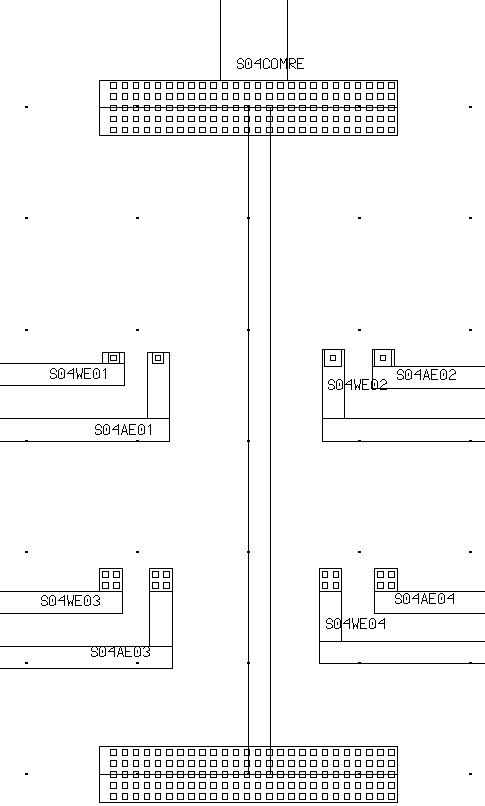
\includegraphics[width=0.6\linewidth]{figures/s04.png}
		\caption{Sensor 4}
		\label{s04}
	\end{minipage}
	\begin{minipage}{0.5\linewidth}
		\centering
		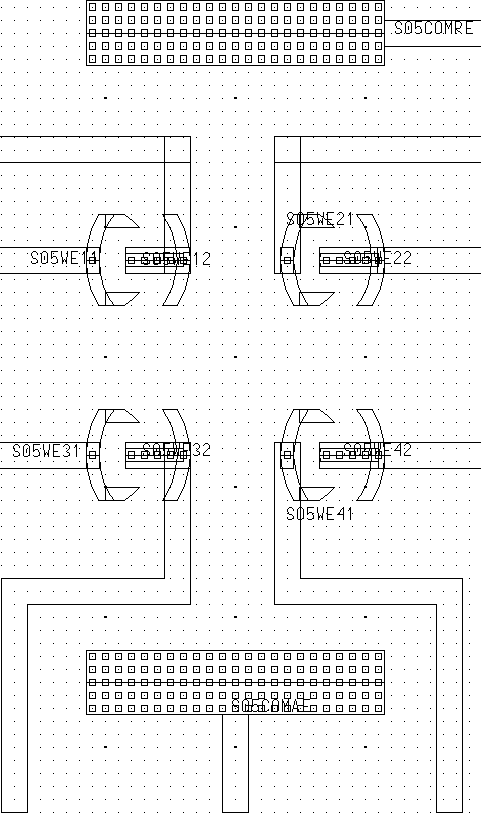
\includegraphics[width=0.6\linewidth]{figures/s05.png}
		\caption{Sensor 5}
		\label{s05}
	\end{minipage}
\end{figure}

\item[Sensor 6] is a 4-electrode system, shape inverse C, with a common RE at top, common AE at bottom (Figure \ref{s06}). WEs 11, 12, 21, 22 are 35.54 $\mu \mathrm{m}$ from the AE. WEs 31, 32, 41, 42 are 15.51 $\mu \mathrm{m}$ from the AE. Pitch is $20 \mu \mathrm{m}$.
\item[Sensor 7] is a 4-electrode system, shape inverse C, with a common RE at top, common AE at bottom (Figure \ref{s07}). WEs 11, 12, 21, 22 are 45.48 $\mu \mathrm{m}$ from the AE. WEs 31, 32, 41, 42 are 20.40 $\mu \mathrm{m}$ from the AE. Pitch is $25 \mu \mathrm{m}$.

\begin{figure}
	\begin{minipage}{0.5\linewidth}
		\centering
		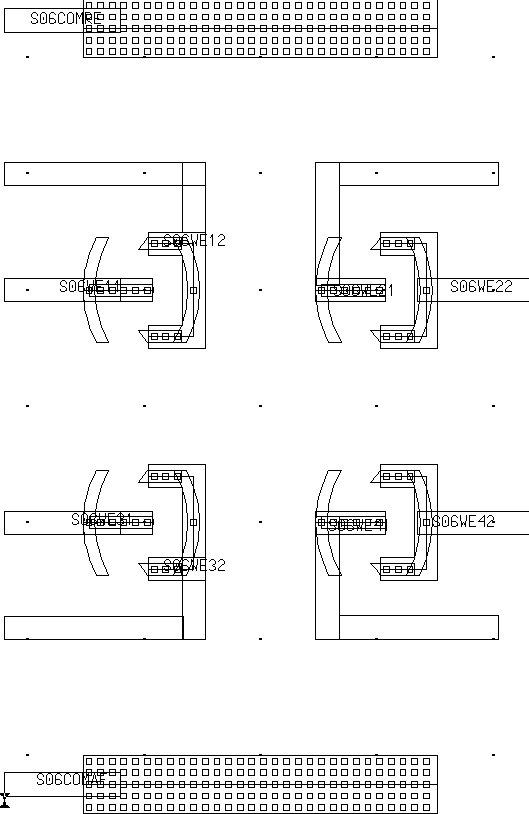
\includegraphics[width=0.6\linewidth]{figures/s06.png}
		\caption{Sensor 6}
		\label{s06}
	\end{minipage}
	\begin{minipage}{0.5\linewidth}
		\centering
		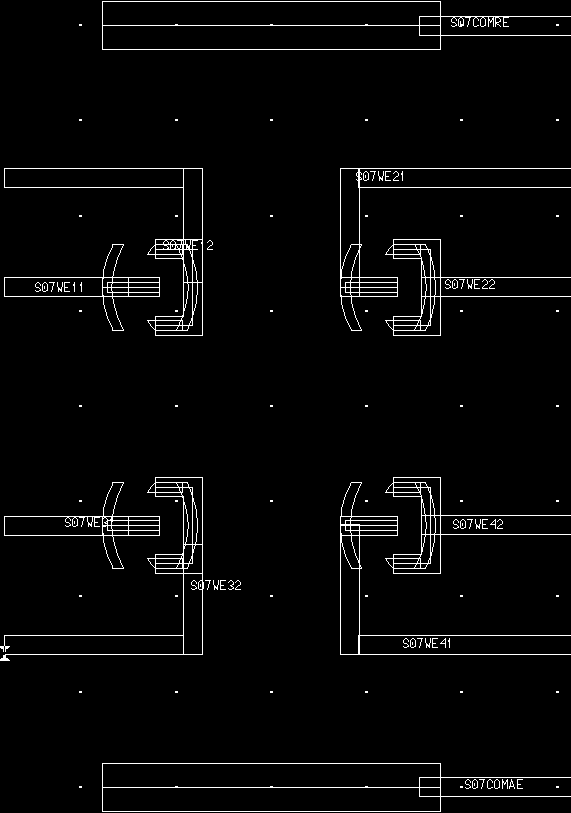
\includegraphics[width=0.6\linewidth]{figures/s07.png}
		\caption{Sensor 7}
		\label{s07}
	\end{minipage}
\end{figure}

\item[Sensor 8] is a 4-electrode system, shape F, with a common RE at top, common AE at bottom (Figure \ref{s08}). WEs 11, 12, 21, 22 are 33.53 $\mu \mathrm{m}$ from the AE. WEs 31, 32, 41, 42 are 13.53 $\mu \mathrm{m}$ from the AE. Pitch is $20 \mu \mathrm{m}$.
\item[Sensor 9] is the same as Sensor 3 (Figure \ref{s09}), but with a pitch of $25 \mu \mathrm{m}$.

\begin{figure}
	\begin{minipage}{0.5\linewidth}
		\centering
		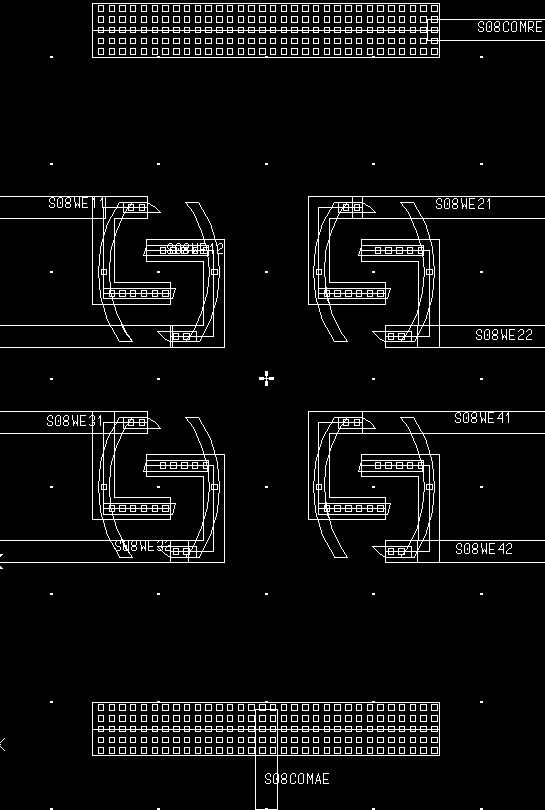
\includegraphics[width=0.6\linewidth]{figures/s08.png}
		\caption{Sensor 8}
		\label{s08}
	\end{minipage}
	\begin{minipage}{0.5\linewidth}
		\centering
		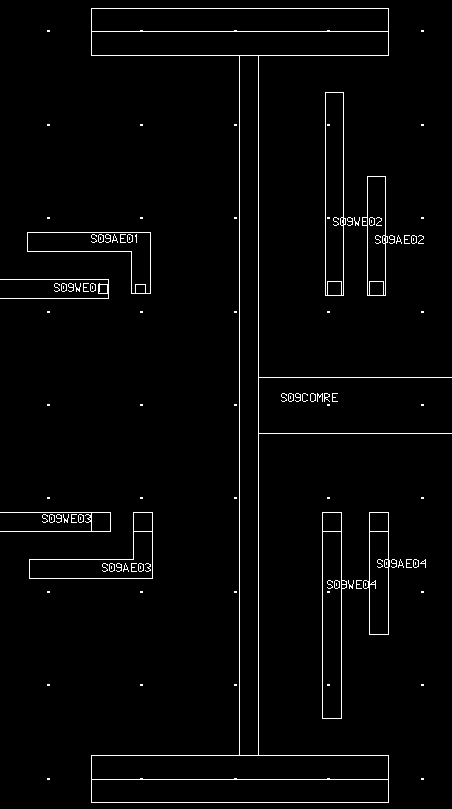
\includegraphics[width=0.6\linewidth]{figures/s09.png}
		\caption{Sensor 9}
		\label{s09}
	\end{minipage}
\end{figure}

\item[Sensor 10] is a 4-electrode system, shape inverse C, with a common RE at top, common AE on 3 sides (Figure \ref{s10}). WEs are 11.50 $\mu \mathrm{m}$ from the AE. Pitch is $15 \mu \mathrm{m}$.
\item[Sensor 11] is a 3-electrode system, with a common RE at top, common AE on 3 sides (Figure \ref{s11}). WEs 1, 2, 3, 4 are 14.47, 14.24, 13.96, 13.96 $\mu \mathrm{m}$ from the AE, respectively. Pitch is $15 \mu \mathrm{m}$.

\begin{figure}
	\begin{minipage}{0.5\linewidth}
		\centering
		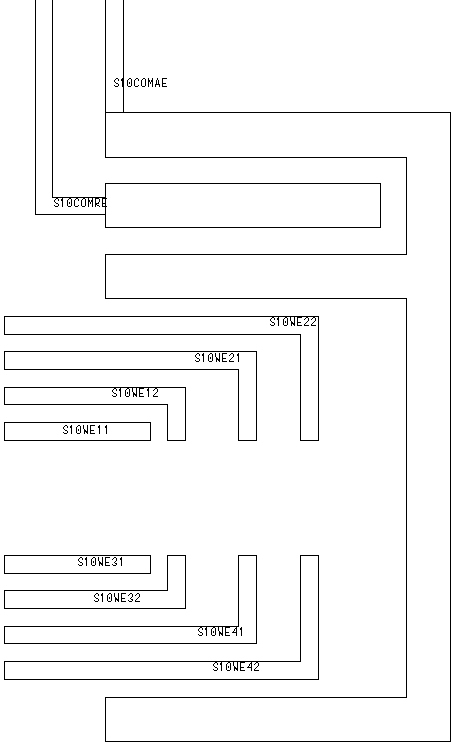
\includegraphics[width=0.6\linewidth]{figures/s10.png}
		\caption{Sensor 10}
		\label{s10}
	\end{minipage}
	\begin{minipage}{0.5\linewidth}
		\centering
		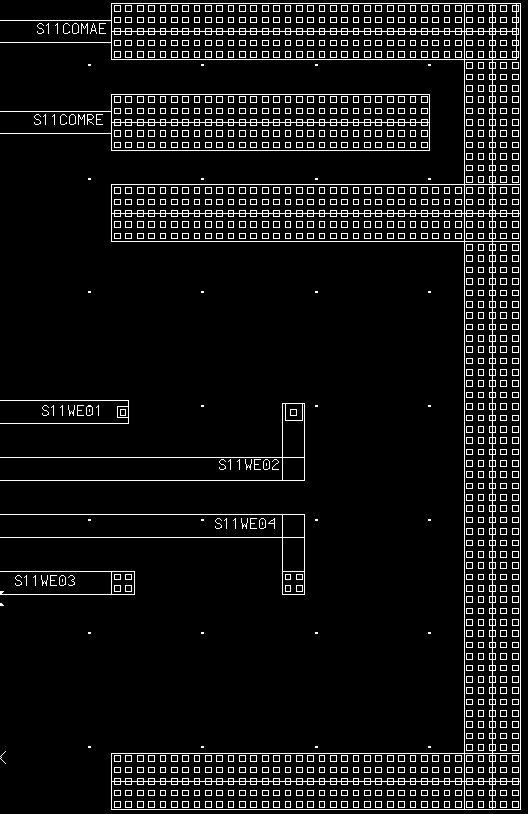
\includegraphics[width=0.6\linewidth]{figures/s11.png}
		\caption{Sensor 11}
		\label{s11}
	\end{minipage}
\end{figure}

\item[Sensor 12] is a 3-electrode system, with a common RE at top, common AE on 3 sides (Figure \ref{s12}). WEs 1, 2, 3, 4 are 19.5, 19.21, 18.98, 18.98 $\mu \mathrm{m}$ from the AE, respectively. Pitch is $20 \mu \mathrm{m}$.
\item[Sensor 13] is a 3-electrode system, with a common RE at top, common AE on 3 sides (Figure \ref{s13}). WEs 1, 2, 3, 4 are 24.53, 24.26, 24.05, 24.05 $\mu \mathrm{m}$ from the AE, respectively. Pitch is $25 \mu \mathrm{m}$.

\begin{figure}
	\begin{minipage}{0.5\linewidth}
		\centering
		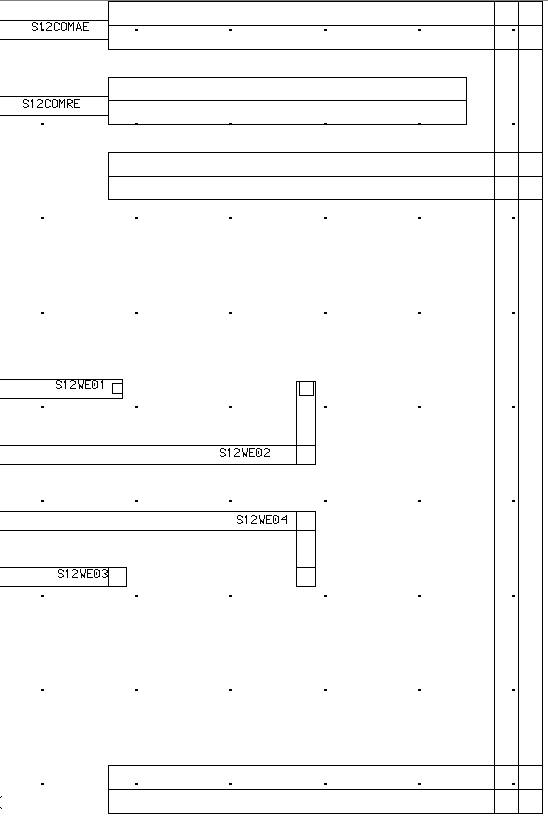
\includegraphics[width=0.6\linewidth]{figures/s12.png}
		\caption{Sensor 12}
		\label{s12}
	\end{minipage}
	\begin{minipage}{0.5\linewidth}
		\centering
		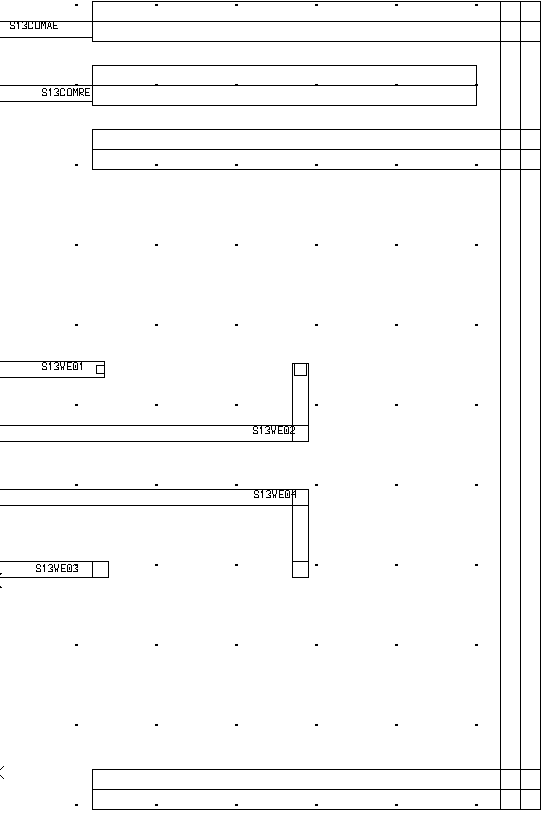
\includegraphics[width=0.6\linewidth]{figures/s13.png}
		\caption{Sensor 13}
		\label{s13}
	\end{minipage}
\end{figure}

\item[Sensor 14] is a 4-electrode system, shape C, with a common RE at top, common AE on 3 sides (Figure \ref{s14}). WEs are 20.50 $\mu \mathrm{m}$ from the AE. Pitch is $25 \mu \mathrm{m}$.
\item[Sensor 15] is a 4-electrode system, shape C, with a common RE at top, common AE on 3 sides (Figure \ref{s15}). WEs are 15.50 $\mu \mathrm{m}$ from the AE. Pitch is $20 \mu \mathrm{m}$.

\begin{figure}
	\begin{minipage}{0.5\linewidth}
		\centering
		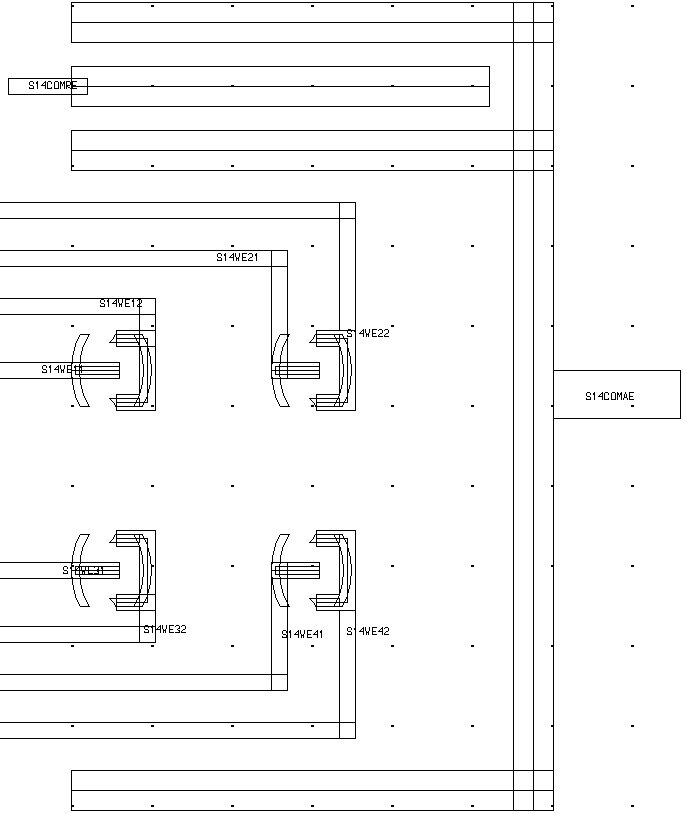
\includegraphics[width=0.6\linewidth]{figures/s14.png}
		\caption{Sensor 14}
		\label{s14}
	\end{minipage}
	\begin{minipage}{0.5\linewidth}
		\centering
		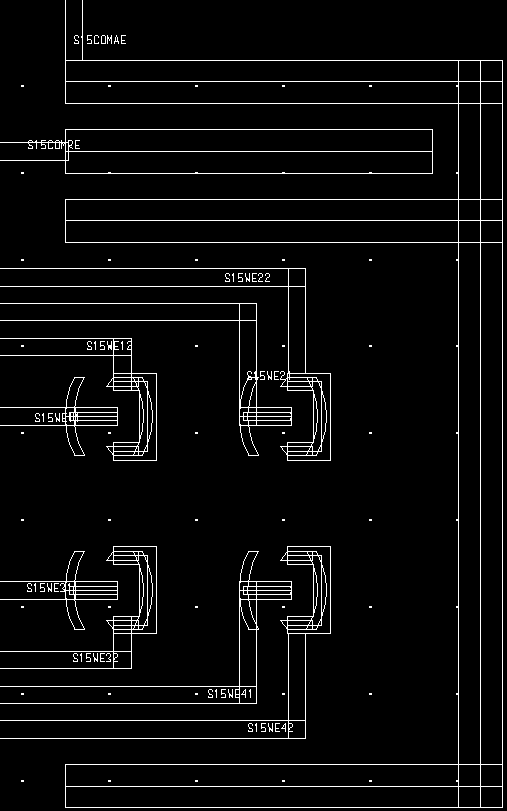
\includegraphics[width=0.6\linewidth]{figures/s15.png}
		\caption{Sensor 15}
		\label{s15}
	\end{minipage}
\end{figure}

\item[Sensor 16] is a 4-electrode system, shape F, with a common RE at top, common AE on 3 sides (Figure \ref{s16}). WEs are 13.50 $\mu \mathrm{m}$ from the AE. Pitch is $20 \mu \mathrm{m}$.
\item[Sensor 17] is a 4-electrode system, shape inverse C, with a common RE at top, common AE at bottom (Figure \ref{s17}). WEs 11, 12, 21, 22 are 43.47 $\mu \mathrm{m}$ from the AE. WEs 31, 32, 41, 42 are 18.46 $\mu \mathrm{m}$ from the AE. Pitch is $25 \mu \mathrm{m}$.

\begin{figure}
	\begin{minipage}{0.5\linewidth}
		\centering
		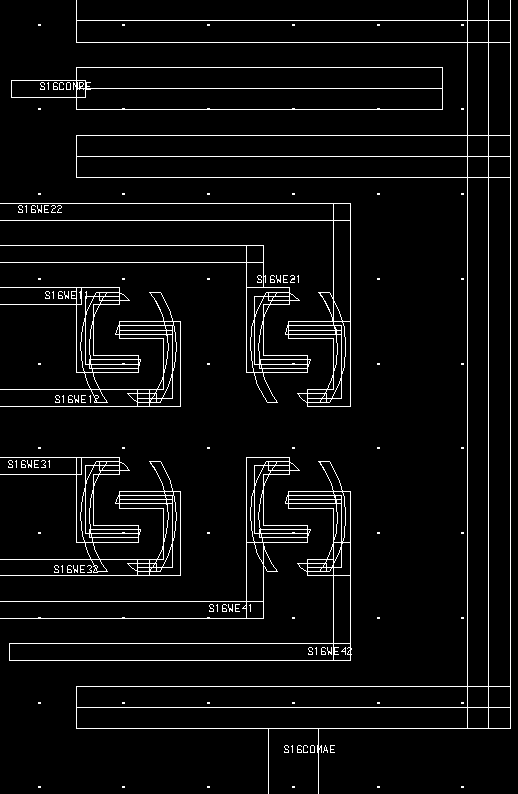
\includegraphics[width=0.6\linewidth]{figures/s16.png}
		\caption{Sensor 16}
		\label{s16}
	\end{minipage}
	\begin{minipage}{0.5\linewidth}
		\centering
		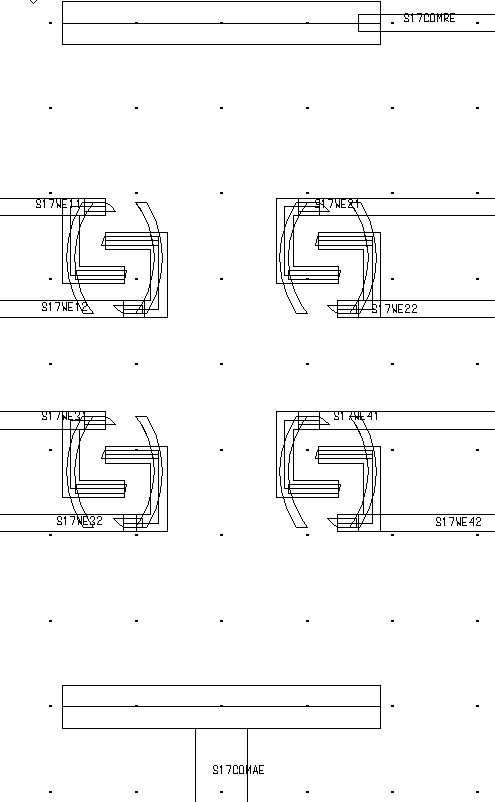
\includegraphics[width=0.6\linewidth]{figures/s17.png}
		\caption{Sensor 17}
		\label{s17}
	\end{minipage}
\end{figure}

\item[Sensor 18] is a 4-electrode system, shape F, with a common RE at top, common AE on 3 sides (Figure \ref{s18}). WEs are 18.50 $\mu \mathrm{m}$ from the AE. Pitch is $25 \mu \mathrm{m}$.
\item[Sensor 19] is the same as Sensor 3 (Figure \ref{s19}), but with a pitch of $15 \mu \mathrm{m}$.

\begin{figure}
	\begin{minipage}{0.5\linewidth}
		\centering
		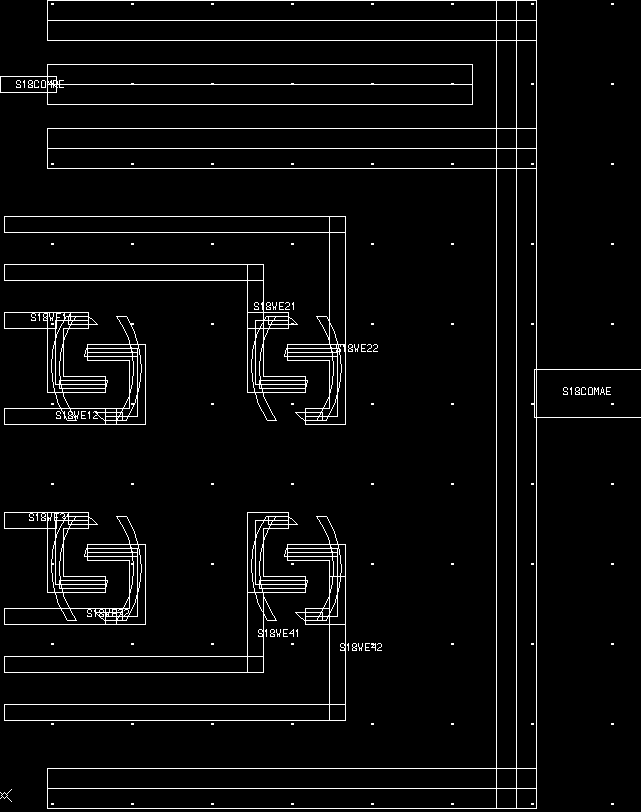
\includegraphics[width=0.6\linewidth]{figures/s18.png}
		\caption{Sensor 18}
		\label{s18}
	\end{minipage}
	\begin{minipage}{0.5\linewidth}
		\centering
		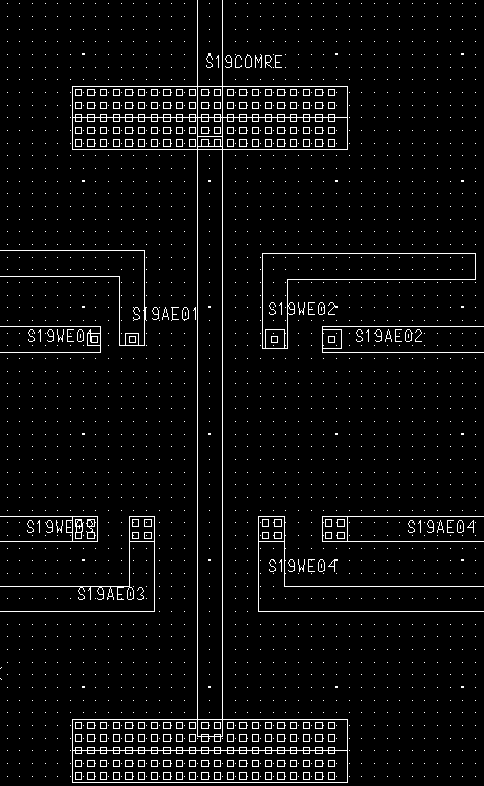
\includegraphics[width=0.6\linewidth]{figures/s19.png}
		\caption{Sensor 19}
		\label{s19}
	\end{minipage}
\end{figure}

\item[Sensor 20] is the same as Sensor 0, except the first WE area has spacing 2 $\mu \mathrm{m}$ (Figure \ref{s20}) and with a pitch of $15 \mu \mathrm{m}$.

\begin{figure}
	\centering
	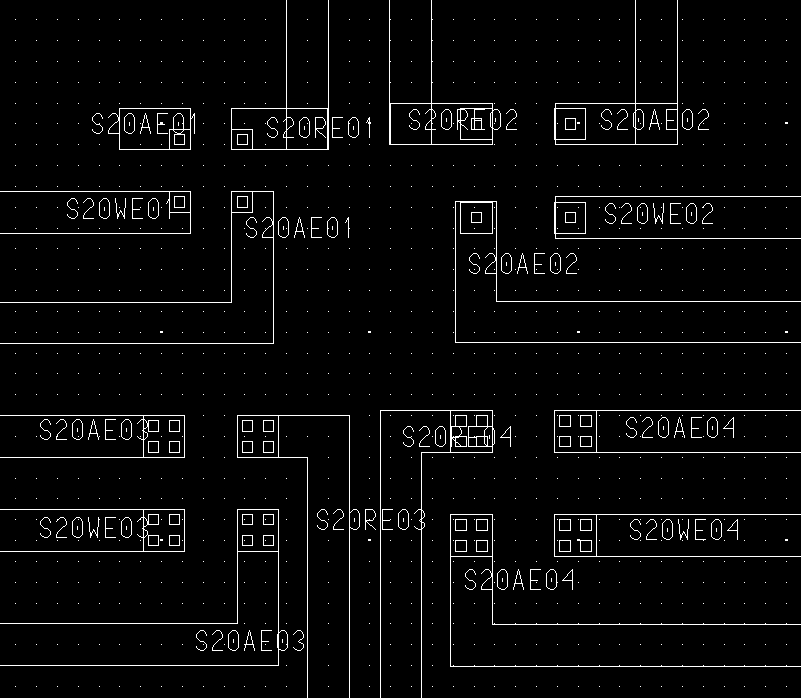
\includegraphics[width=0.3\linewidth]{figures/s20.png}
	\caption{Sensor 20}
	\label{s20}
\end{figure}

\end{description}

\begin{table}
	\begin{tabular}{p{4cm}|p{2cm}|p{2cm}|p{2.5cm}|p{2cm}}
		electrode system: & \textbf{3} & \textbf{4, C} & \textbf{4, inverse C} & \textbf{4, F} \\
		\hline
		\textbf{2 auxiliary} & 0, 1, 2, 20 & & & \\
		\hline
		\textbf{common reference, top \& bottom} & 3, 4, 9, 19 & & & \\
		\hline
		\textbf{common reference top, common auxiliary bottom} & & 5 & 6, 7 & 8, 17 \\
		\hline
		\textbf{common reference top, common auxiliary on 3 sides} & 11, 12, 13 & 14, 15 & 10 & 16, 18
	\end{tabular}
	\caption{Sensor site configurations}
	\label{sensor-config}
\end{table}

These data, including areas and perimeters of AEs, are summarized in Table \ref{electrode-properties-1}, \ref{electrode-properties-2}, \ref{electrode-properties-3}.

\begin{table}
	\begin{tabular}{lllllll}
		sensor & WE & area & perimeter & WE distance to AE & AE area & AE perimeter \\
		\hline
		0 & 1 & 1 & 4 & 3 & 1 & 4 \\
		0 & 2 & 2.25 & 6 & 3 & 2.25 & 6 \\
		0 & 3 & 4 & 8 & 2.5 & 4 & 8 \\
		0 & 4 & 4 & 8 & 3 & 4 & 8 \\
		1 & 1 & 1 & 4 & 3 & 1 & 4 \\
		1 & 2 & 2.25 & 6 & 3 & 2.25 & 6 \\
		1 & 3 & 4 & 8 & 2.5 & 4 & 8 \\
		1 & 4 & 4 & 8 & 3 & 4 & 8 \\
		2 & 1 & 1 & 4 & 3 & 1 & 4 \\
		2 & 2 & 2.25 & 6 & 3 & 2.25 & 6 \\
		2 & 3 & 4 & 8 & 2.5 & 4 & 8 \\
		2 & 4 & 4 & 8 & 3 & 4 & 8 \\
		3 & 1 & 1 & 4 & 3 & 1 & 4 \\
		3 & 2 & 2.25 & 6 & 3 & 2.25 & 6 \\
		3 & 3 & 4 & 8 & 2.5 & 4 & 8 \\
		3 & 4 & 4 & 8 & 3 & 4 & 8 \\
		4 & 1 & 1 & 4 & 3 & 1 & 4 \\
		4 & 2 & 2.25 & 6 & 3 & 2.25 & 6 \\
		4 & 3 & 4 & 8 & 2.5 & 4 & 8 \\
		4 & 4 & 4 & 8 & 3 & 4 & 8 \\
		5 & 11 & 10.885 & 24.7 & 26.55 & 115 & 56 \\
		5 & 12 & 11.342 & 25.081 & 26.55 & 115 & 56 \\
		5 & 21 & 10.885 & 24.7 & 26.55 & 115 & 56 \\
		5 & 22 & 11.342 & 25.081 & 26.55 & 115 & 56 \\
		5 & 31 & 10.885 & 24.7 & 11.51 & 115 & 56 \\
		5 & 32 & 11.342 & 25.081 & 11.51 & 115 & 56 \\
		5 & 41 & 10.885 & 24.7 & 11.51 & 115 & 56 \\
		5 & 42 & 11.342 & 25.081 & 11.51 & 115 & 56 \\
		6 & 11 & 14.267 & 30.793 & 35.54 & 152.5 & 71 \\
		6 & 12 & 15.119 & 32.835 & 35.54 & 152.5 & 71 \\
		6 & 21 & 14.267 & 30.793 & 35.54 & 152.5 & 71 \\
		6 & 22 & 15.119 & 32.835 & 35.54 & 152.5 & 71 \\
		6 & 31 & 14.267 & 30.793 & 15.51 & 152.5 & 71 \\
		6 & 32 & 15.119 & 32.835 & 15.51 & 152.5 & 71 \\
		6 & 41 & 14.267 & 30.793 & 15.51 & 152.5 & 71 \\
		6 & 42 & 15.119 & 32.835 & 15.51 & 152.5 & 71 \\
		7 & 11 & 14.267 & 30.793 & 45.48 & 177.5 & 81 \\
		7 & 12 & 15.119 & 32.835 & 45.48 & 177.5 & 81 \\
		7 & 21 & 14.267 & 30.793 & 45.48 & 177.5 & 81 \\
		7 & 22 & 15.119 & 32.835 & 45.48 & 177.5 & 81 \\
		7 & 31 & 14.267 & 30.793 & 20.4 & 177.5 & 81 \\
		7 & 32 & 15.119 & 32.835 & 20.4 & 177.5 & 81 \\
		7 & 41 & 14.267 & 30.793 & 20.4 & 177.5 & 81 \\
		7 & 42 & 15.119 & 32.835 & 20.4 & 177.5 & 81
	\end{tabular}
	\caption[Electrode properties for sensors 0--7]{Electrode properties for sensors 0--7. Areas are in $\mu \mathrm{m}^2$. Perimeters and distances are in $\mu \mathrm{m}$. WE distance to AE lists shortest distance between the two electrodes.}
	\label{electrode-properties-1}
\end{table}

\begin{table}
	\begin{tabular}{lllllll}
		sensor & WE & WE area & WE perimeter & WE distance to AE & AE area & AE perimeter \\
		\hline
		8 & 11 & 21.771 & 46.636 & 33.53 & 161.25 & 74.5 \\
		8 & 12 & 21.738 & 46.796 & 33.53 & 161.25 & 74.5 \\
		8 & 21 & 21.771 & 46.636 & 33.53 & 161.25 & 74.5 \\
		8 & 22 & 21.738 & 46.796 & 33.53 & 161.25 & 74.5 \\
		8 & 31 & 21.771 & 46.636 & 13.53 & 161.25 & 74.5 \\
		8 & 32 & 21.738 & 46.796 & 13.53 & 161.25 & 74.5 \\
		8 & 41 & 21.771 & 46.636 & 13.53 & 161.25 & 74.5 \\
		8 & 42 & 21.738 & 46.796 & 13.53 & 161.25 & 74.5 \\
		9 & 1 & 1 & 4 & 3 & 1 & 4 \\
		9 & 2 & 2.25 & 6 & 3 & 2.25 & 6 \\
		9 & 3 & 4 & 8 & 2.5 & 4 & 8 \\
		9 & 4 & 4 & 8 & 3 & 4 & 8 \\
		10 & 11 & 14.267 & 30.793 & 11.5 & 865 & 356 \\
		10 & 12 & 15.119 & 32.835 & 11.5 & 865 & 356 \\
		10 & 21 & 14.267 & 30.793 & 11.5 & 865 & 356 \\
		10 & 22 & 15.119 & 32.835 & 11.5 & 865 & 356 \\
		10 & 31 & 14.267 & 30.793 & 11.5 & 865 & 356 \\
		10 & 32 & 15.119 & 32.835 & 11.5 & 865 & 356 \\
		10 & 41 & 14.267 & 30.793 & 11.5 & 865 & 356 \\
		10 & 42 & 15.119 & 32.835 & 11.5 & 865 & 356 \\
		11 & 1 & 1 & 4 & 14.47 & 820 & 338 \\
		11 & 2 & 2.25 & 6 & 14.24 & 820 & 338 \\
		11 & 3 & 4 & 8 & 13.96 & 820 & 338 \\
		11 & 4 & 4 & 8 & 13.96 & 820 & 338 \\
		12 & 1 & 1 & 4 & 19.5 & 1045 & 428 \\
		12 & 2 & 2.25 & 6 & 19.21 & 1045 & 428 \\
		12 & 3 & 4 & 8 & 18.98 & 1045 & 428 \\
		12 & 4 & 4 & 8 & 18.98 & 1045 & 428 \\
		13 & 1 & 1 & 4 & 24.53 & 1270 & 518 \\
		13 & 2 & 2.25 & 6 & 24.26 & 1270 & 518 \\
		13 & 3 & 4 & 8 & 24.05 & 1270 & 518 \\
		13 & 4 & 4 & 8 & 24.05 & 1270 & 518 \\
		14 & 11 & 10.885 & 24.7 & 20.5 & 1333.75 & 543.5 \\
		14 & 12 & 11.342 & 25.081 & 20.5 & 1333.75 & 543.5 \\
		14 & 21 & 10.885 & 24.7 & 20.5 & 1333.75 & 543.5 \\
		14 & 22 & 11.342 & 25.081 & 20.5 & 1333.75 & 543.5 \\
		14 & 31 & 10.885 & 24.7 & 20.5 & 1333.75 & 543.5 \\
		14 & 32 & 11.342 & 25.081 & 20.5 & 1333.75 & 543.5 \\
		14 & 41 & 10.885 & 24.7 & 20.5 & 1333.75 & 543.5 \\
		14 & 42 & 11.342 & 25.081 & 20.5 & 1333.75 & 543.5
	\end{tabular}
	\caption[Electrode properties for sensors 8--14]{Electrode properties for sensors 8--14. Areas are in $\mu \mathrm{m}^2$. Perimeters and distances are in $\mu \mathrm{m}$. WE distance to AE lists shortest distance between the two electrodes.}
	\label{electrode-properties-2}
\end{table}

\begin{table}
	\begin{tabular}{lllllll}
		sensor & WE & area & perimeter & WE distance to AE & AE area & AE perimeter \\
		\hline
		15 & 11 & 10.885 & 24.7 & 15.5 & 1108.75 & 453.5 \\
		15 & 12 & 11.342 & 25.081 & 15.5 & 1108.75 & 453.5 \\
		15 & 21 & 10.885 & 24.7 & 15.5 & 1108.75 & 453.5 \\
		15 & 22 & 11.342 & 25.081 & 15.5 & 1108.75 & 453.5 \\
		15 & 31 & 10.885 & 24.7 & 15.5 & 1108.75 & 453.5 \\
		15 & 32 & 11.342 & 25.081 & 15.5 & 1108.75 & 453.5 \\
		15 & 41 & 10.885 & 24.7 & 15.5 & 1108.75 & 453.5 \\
		15 & 42 & 11.342 & 25.081 & 15.5 & 1108.75 & 453.5 \\
		16 & 11 & 21.771 & 46.636 & 13.5 & 1121.875 & 458.75 \\
		16 & 12 & 21.738 & 46.796 & 13.5 & 1121.875 & 458.75 \\
		16 & 21 & 21.771 & 46.636 & 13.5 & 1121.875 & 458.75 \\
		16 & 22 & 21.738 & 46.796 & 13.5 & 1121.875 & 458.75 \\
		16 & 31 & 21.771 & 46.636 & 13.5 & 1121.875 & 458.75 \\
		16 & 32 & 21.738 & 46.796 & 13.5 & 1121.875 & 458.75 \\
		16 & 41 & 21.771 & 46.636 & 13.5 & 1121.875 & 458.75 \\
		16 & 42 & 21.738 & 46.796 & 13.5 & 1121.875 & 458.75 \\
		17 & 11 & 14.267 & 30.793 & 43.47 & 186.25 & 84.5 \\
		17 & 12 & 15.119 & 32.835 & 43.47 & 186.25 & 84.5 \\
		17 & 21 & 14.267 & 30.793 & 43.47 & 186.25 & 84.5 \\
		17 & 22 & 15.119 & 32.835 & 43.47 & 186.25 & 84.5 \\
		17 & 31 & 14.267 & 30.793 & 18.46 & 186.25 & 84.5 \\
		17 & 32 & 15.119 & 32.835 & 18.46 & 186.25 & 84.5 \\
		17 & 41 & 14.267 & 30.793 & 18.46 & 186.25 & 84.5 \\
		17 & 42 & 15.119 & 32.835 & 18.46 & 186.25 & 84.5 \\
		18 & 11 & 21.771 & 46.636 & 18.5 & 1346.875 & 548.75 \\
		18 & 12 & 21.738 & 46.796 & 18.5 & 1346.875 & 548.75 \\
		18 & 21 & 21.771 & 46.636 & 18.5 & 1346.875 & 548.75 \\
		18 & 22 & 21.738 & 46.796 & 18.5 & 1346.875 & 548.75 \\
		18 & 31 & 21.771 & 46.636 & 18.5 & 1346.875 & 548.75 \\
		18 & 32 & 21.738 & 46.796 & 18.5 & 1346.875 & 548.75 \\
		18 & 41 & 21.771 & 46.636 & 18.5 & 1346.875 & 548.75 \\
		18 & 42 & 21.738 & 46.796 & 18.5 & 1346.875 & 548.75 \\
		19 & 1 & 1 & 4 & 2 & 1 & 4 \\
		19 & 2 & 2.25 & 6 & 3 & 2.25 & 6 \\
		19 & 3 & 4 & 8 & 2.5 & 4 & 8 \\
		19 & 4 & 4 & 8 & 3 & 4 & 8 \\
		20 & 1 & 1 & 4 & 2 & 1 & 4 \\
		20 & 2 & 2.25 & 6 & 3 & 2.25 & 6 \\
		20 & 3 & 4 & 8 & 2.5 & 4 & 8 \\
		20 & 4 & 4 & 8 & 3 & 4 & 8
	\end{tabular}
	\caption[Electrode properties for sensors 15--20]{Electrode properties for sensors 15--20. Areas are in $\mu \mathrm{m}^2$. Perimeters and distances are in $\mu \mathrm{m}$. WE distance to AE lists shortest distance between the two electrodes.}
	\label{electrode-properties-3}
\end{table}

\section{Experiment Setup}

A CH Instruments 660B potentiostat was used to perform all tests. A PDMS well was attached to the chip to prevent solutions from leaking onto probe pads (Figure \ref{chip-top}). The chip was mounted onto a probestation, which was shielded by enclosing it in a Faraday cage (Figure \ref{probestation}). Pins were lowered onto the probe-pads of the chip (Figure \ref{chippins}, \ref{chippins-top}), which were connected to the reference, auxiliary, and working electrode leads of the potentiostat (Figure \ref{potentiostatleads}).

\begin{figure}
	\centering
	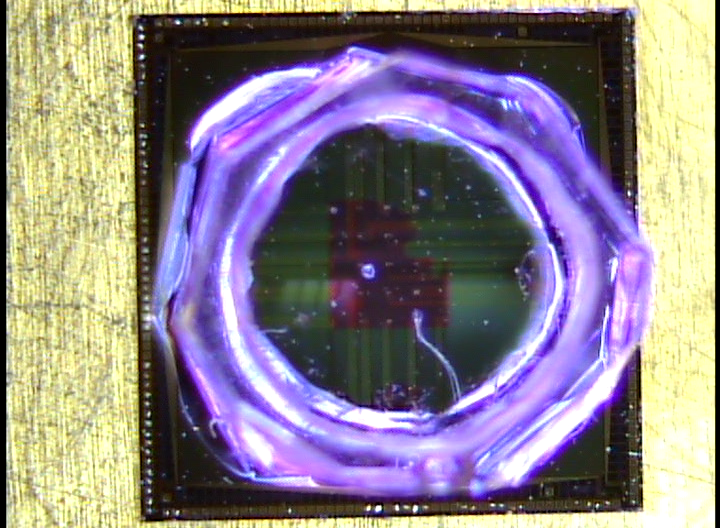
\includegraphics[width=0.5\linewidth]{figures/chip-top.png}
	\caption{Chip with PDMS well attached}
	\label{chip-top}
\end{figure}

\begin{figure}
	\centering
	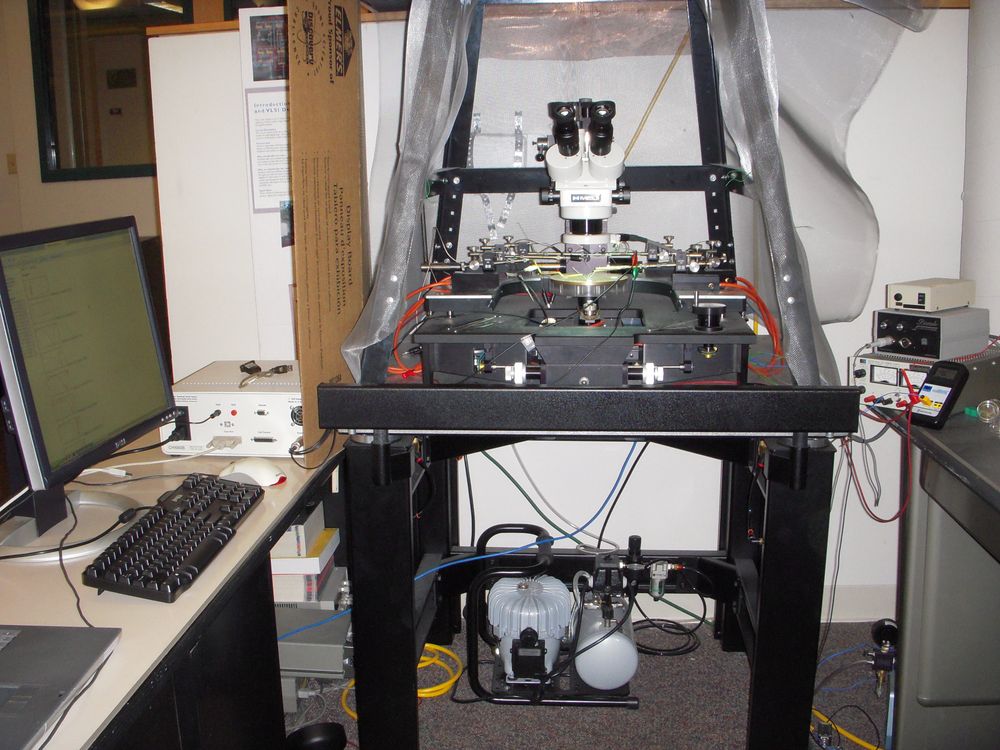
\includegraphics[width=0.5\linewidth]{figures/probestation.png}
	\caption[Probestation]{Probestation enclosed in a Faraday cage, and connected to the potentiostat}
	\label{probestation}
\end{figure}

\begin{figure}
	\centering
	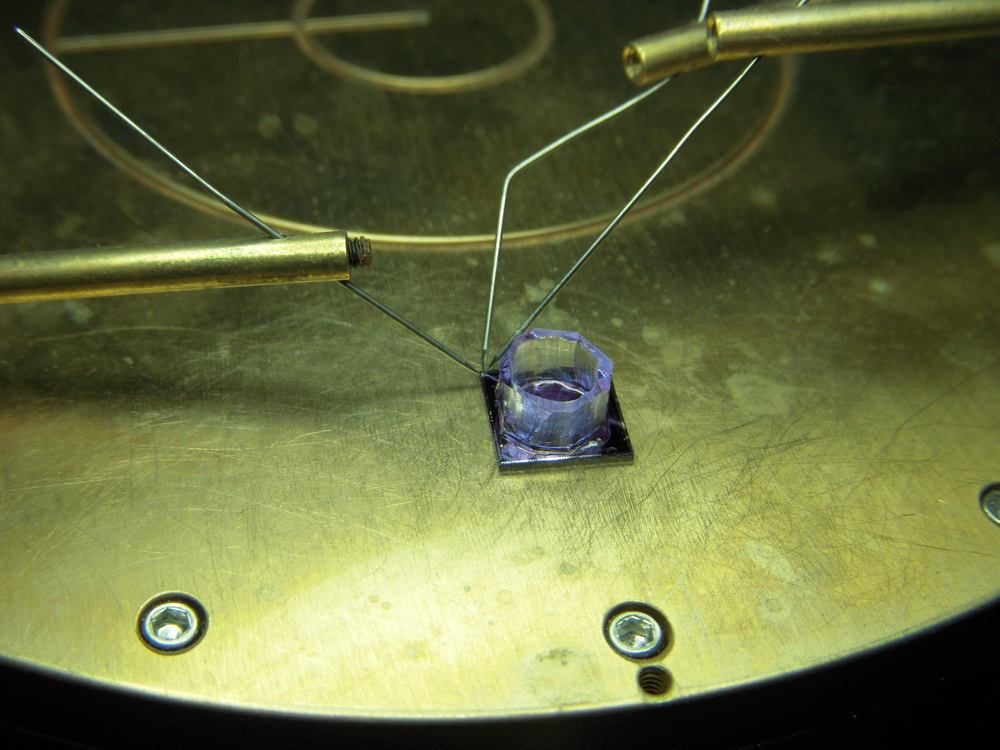
\includegraphics[width=0.5\linewidth]{figures/chippins.png}
	\caption{Pins lowered onto probe pads of the chip}
	\label{chippins}
\end{figure}

\begin{figure}
	\centering
	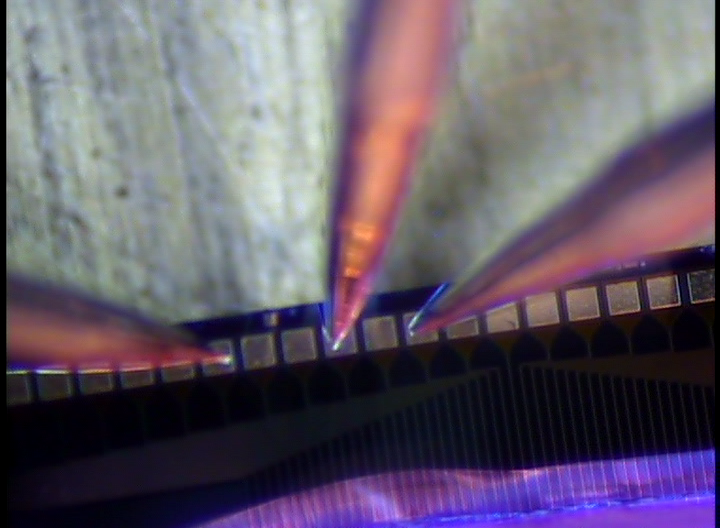
\includegraphics[width=0.5\linewidth]{figures/chippins-top.png}
	\caption{Pins lowered onto probe pads of the chip, top view}
	\label{chippins-top}
\end{figure}

\begin{figure}
	\centering
	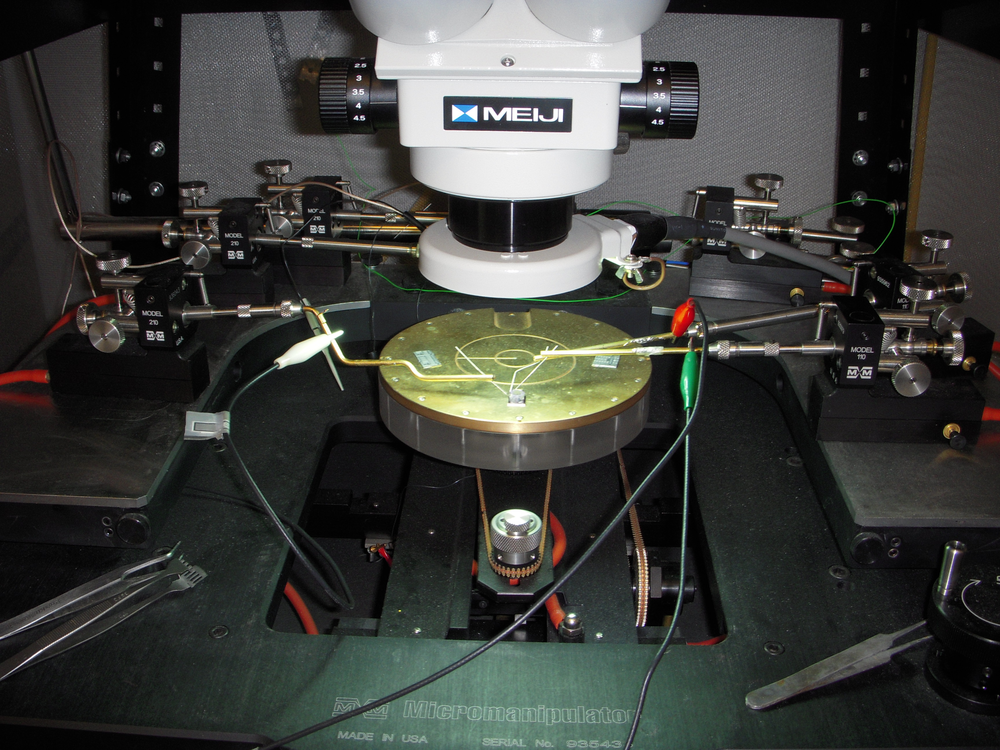
\includegraphics[width=0.5\linewidth]{figures/potentiostatleads.png}
	\caption[Potentiostat leads connected to pins]{Potentiostat leads for reference, auxiliary, and working electrodes connected to chip pins (white, red, and green, respectively)}
	\label{potentiostatleads}
\end{figure}

\section{Experiment Procedure}

The 21 sensor sites were characterized to find the best general electrode construction. This was done using DPV and varying the electrodes and solution concentrations.

\subsection{All Sites}

The first set of tests was done by performing DPV from -0.2V to 0.2V on two randomly-chosen WE areas of each sensor site, three times each (six tests on each sensor site). The solution used was 0.3mM NE in 0.1M $\mathrm{H}_2\mathrm{SO}_4$. Before a WE area was used, it was cleaned by CV from -0.3V to 1.5V at 1V/s with 20 cycles, with a solution of 0.1M $\mathrm{H}_2\mathrm{SO}_4$. The result of each individual test was taken to be the distance of the baseline to the bottom of the peak centered around 0.0V. The result of each sensor site was taken to be the average of the six tests on that site.

\subsection{Limit of Detection}

The second set of tests was done on sensors 17 and 8, which were the two highest-performing sensors from the previous test. The same procedure was used as above, except decreasing concentrations of NE were used.

\subsection{Specific Electrodes}

The third set of tests was done on specific WE areas (instead of randomly chosen areas), based on their performance and our hypotheses about their performance. The procedure used was the same as above, except specific WE areas were chosen, and multiple chips were tested to control against process variation while manufacturing the chips.

\section{Experiment Results}

Results for the first set of tests (all sites) are summarized in Table \ref{dpv-results}. Results for the third set of tests are summarized in Table \ref{dpv-specific}. Below are our hypotheses about electrode configuration, and the results that correspond to those hypotheses.

\begin{table}
	\begin{tabular}{lll}
		Sensor & \% of max & Avg. value \\
		\hline
		17 & 100.0 $\pm$ 4.0 & 7.04e-10 $\pm$ 2.83e-11 \\
		8 & 77.9 $\pm$ 5.5 & 5.48e-10 $\pm$ 3.85e-11 \\
		16 & 75.7 $\pm$ 1.8 & 5.32e-10 $\pm$ 1.28e-11 \\
		7 & 71.5 $\pm$ 3.0 & 5.03e-10 $\pm$ 2.13e-11 \\
		18 & 58.8 $\pm$ 2.5 & 4.14e-10 $\pm$ 1.73e-11 \\
		6 & 57.6 $\pm$ 4.0 & 4.05e-10 $\pm$ 2.79e-11 \\
		15 & 55.2 $\pm$ 3.5 & 3.89e-10 $\pm$ 2.43e-11 \\
		14 & 50.8 $\pm$ 2.1 & 3.57e-10 $\pm$ 1.46e-11 \\
		10 & 47.6 $\pm$ 3.6 & 3.35e-10 $\pm$ 2.50e-11 \\
		5 & 43.0 $\pm$ 1.2 & 3.03e-10 $\pm$ 8.27e-12 \\
		1 & 36.7 $\pm$ 3.5 & 2.58e-10 $\pm$ 2.46e-11 \\
		20 & 26.1 $\pm$ 1.0 & 1.84e-10 $\pm$ 7.29e-12 \\
		0 & 23.8 $\pm$ 5.0 & 1.68e-10 $\pm$ 3.55e-11 \\
		19 & 21.9 $\pm$ 2.0 & 1.54e-10 $\pm$ 1.44e-11 \\
		12 & 19.5 $\pm$ 1.5 & 1.37e-10 $\pm$ 1.05e-11 \\
		4 & 19.2 $\pm$ 1.8 & 1.35e-10 $\pm$ 1.28e-11 \\
		13 & 19.1 $\pm$ 1.0 & 1.34e-10 $\pm$ 7.37e-12 \\
		2 & 17.6 $\pm$ 2.1 & 1.24e-10 $\pm$ 1.49e-11 \\
		9 & 17.5 $\pm$ 0.4 & 1.23e-10 $\pm$ 2.83e-12 \\
		11 & 14.4 $\pm$ 1.9 & 1.01e-10 $\pm$ 1.33e-11 \\
		3 & 11.3 $\pm$ 1.3 & 7.93e-11 $\pm$ 9.48e-12
	\end{tabular}
	\caption[DPV results for sensor sites]{DPV results for sensor sites sorted by decreasing value}
	\label{dpv-results}
\end{table}

\begin{table}
	\begin{tabular}{lllllll}
		sensor & electrode & chip 1 & chip 3 & chip 4 & distance & area \\
		\hline
		02 & 01 &           & 1.493e-10 $\pm$ 7.3e-12 & 1.632e-10 $\pm$ 1.6e-12 &  3.00 & 1 \\
		02 & 02 &           & 1.921e-10 $\pm$ 4.1e-12 & 2.120e-10 $\pm$ 8.9e-12 &  3.00 & 2.25 \\
		02 & 03 &           & 1.940e-10 $\pm$ 1.1e-11 & 2.250e-10 $\pm$ 2.0e-12 &  2.50 & 4 \\
		02 & 04 &           & 1.419e-10 $\pm$ 8.5e-12 & 1.850e-10 $\pm$ 4.6e-12 &  3.00 & 4 \\
		07 & 12 & 5.169e-10 & 4.774e-10 $\pm$ 2.1e-11 & 4.994e-10 $\pm$ 1.2e-11 & 45.48 & 15.119 \\
		07 & 32 & 3.245e-10 & 4.963e-10 $\pm$ 1.1e-11 & 4.072e-10 $\pm$ 2.2e-12 & 20.40 & 15.119 \\
		16 & 12 & 5.157e-10 & 7.212e-10 $\pm$ 2.4e-11 & 6.188e-10 $\pm$ 1.3e-11 & 13.50 & 21.738 \\
		16 & 32 & 6.494e-10 & 6.349e-10 $\pm$ 5.2e-12 & 6.989e-10 $\pm$ 1.0e-11 & 13.50 & 21.738 \\
		17 & 11 & 6.562e-10 &                         &                         & 43.47 & 21.771 \\
		17 & 12 & 4.949e-10 & 5.533e-10 $\pm$ 8.5e-12 & 6.420e-10 $\pm$ 9.2e-12 & 43.47 & 21.738 \\
		17 & 31 & 6.913e-10 &                         &                         & 18.46 & 21.771 \\
		17 & 32 & 6.593e-10 & 6.360e-10 $\pm$ 5.9e-12 & 6.284e-10 $\pm$ 1.2e-11 & 18.46 & 21.738 \\
		18 & 12 & 5.570e-10 & 5.377e-10 $\pm$ 8.8e-12 & 6.130e-10 $\pm$ 8.5e-12 & 18.50 & 21.738 \\
		18 & 32 & 5.683e-10 &                         & 4.965e-10 $\pm$ 2.8e-12 & 18.50 & 21.738
	\end{tabular}
	\caption[Results of further DPV tests on specific working electrodes]{Results of further DPV tests on specific working electrodes. Outputs are given from averaged data from runs on chips 1, 3, and 4 with standard error in amperes. The distance column lists the distance of the working to the auxiliary electrode from Table \ref{electrode-properties-1}, \ref{electrode-properties-2}, \ref{electrode-properties-3} in $\mu \mathrm{m}$. The area column lists the area of the working electrode from Table \ref{WE-size} in $\mu \mathrm{m}^2$. Chip 2 was not performing well and was skipped. Chips 3 and 4 used the same solution. Chip 1 used a separate solution. They were both mixed to be identical, but at concentrations this low, that is difficult to guarantee. Thus, do not use these data without adjusting for relative performance.}
	\label{dpv-specific}
\end{table}

\subsection{Output vs. Working Electrode Area}

This hypothesis is that the output current is proportional to the WE area. Figure \ref{area_v_output} shows all 126 tests and a linear-fit curve. Although there is a large variation in this correlation, it is clear that there is a general trend towards larger WE area leading to greater output, supporting this hypothesis. However, due to variations in sensor configurations, AE areas, perimeters, and distances, there is not much more we can say about this.

\begin{figure}
	\centering
	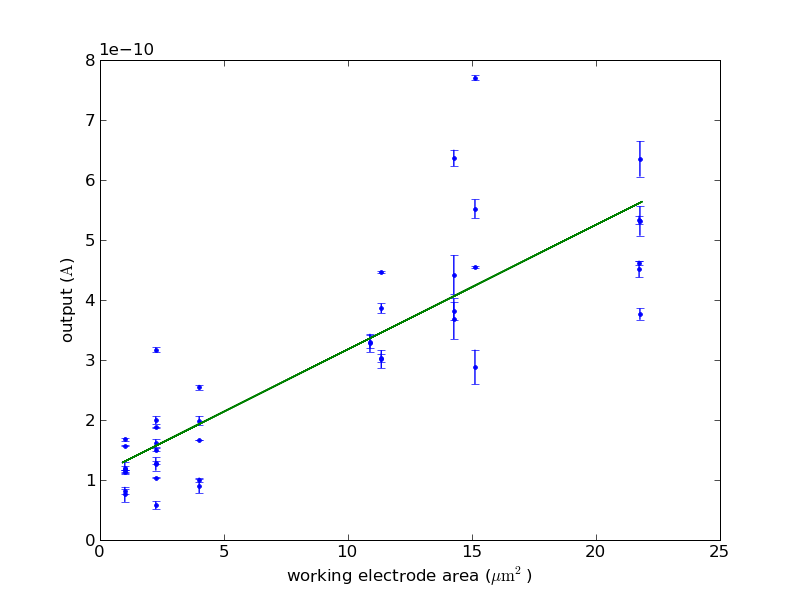
\includegraphics[width=0.7\linewidth]{figures/area_v_output.png}
	\caption{WE area vs. Output}
	\label{area_v_output}
\end{figure}

\subsection{Output Density vs. Working Electrode Area}

This hypothesis is that the output current density is proportional to the WE area. Figure \ref{area_v_density} shows all 126 tests and a linear-fit curve. Here there appears to be a general trend. However, this is likely not the case. The areas above 10 microns are 4-electrode systems; the areas below 10 microns are 3-electrode systems. The two systems differ significantly, so it is reasonable to separate them for analysis. When viewed this way (Figure \ref{area_low_v_density}, \ref{area_high_v_density}), it is clear that there is no conclusive data to support this hypothesis.

\begin{figure}
	\centering
	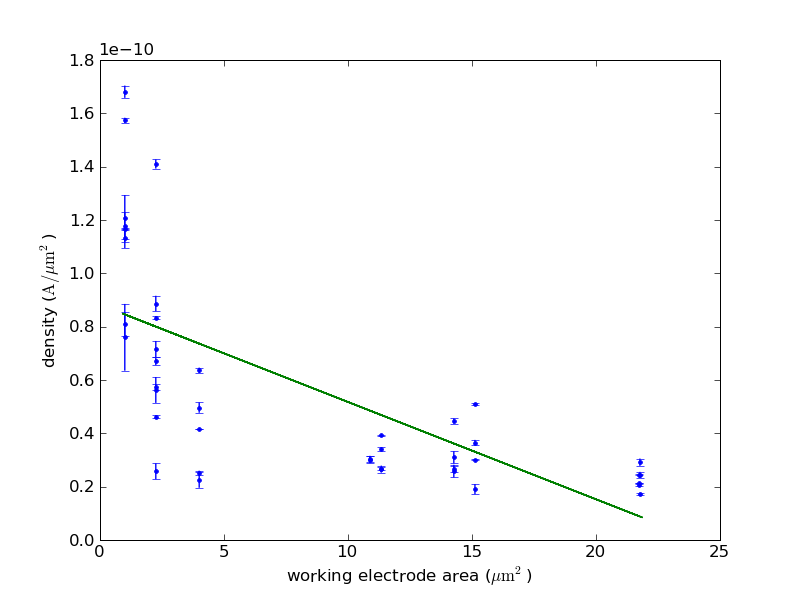
\includegraphics[width=0.7\linewidth]{figures/area_v_density.png}
	\caption{WE area vs. Density}
	\label{area_v_density}
\end{figure}

\begin{figure}
	\centering
	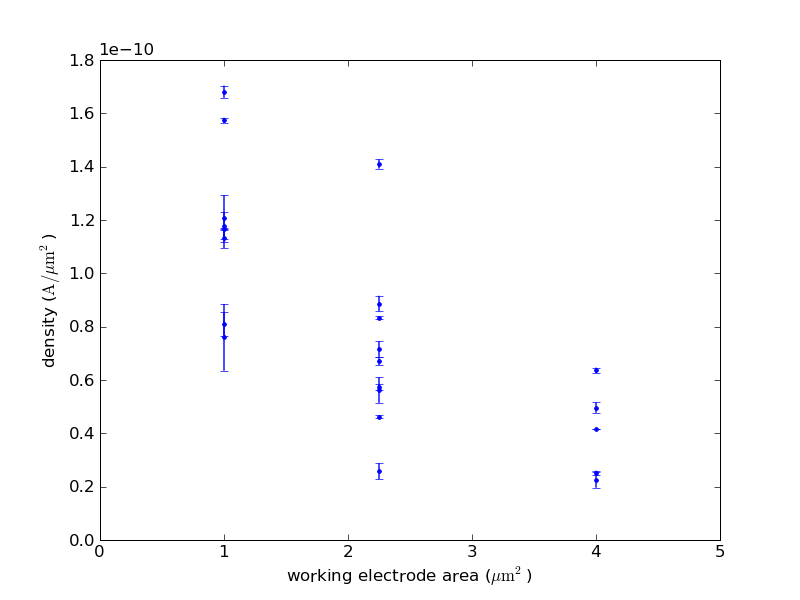
\includegraphics[width=0.7\linewidth]{figures/area_low_v_density.png}
	\caption{WEs with low area vs. Density}
	\label{area_low_v_density}
\end{figure}

\begin{figure}
	\centering
	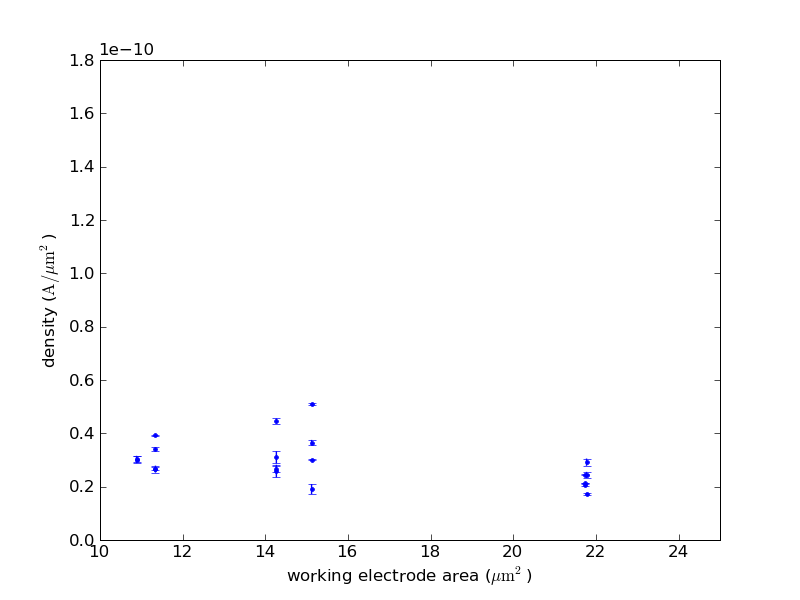
\includegraphics[width=0.7\linewidth]{figures/area_high_v_density.png}
	\caption{WEs with high area vs. Density}
	\label{area_high_v_density}
\end{figure}

\subsection{Ratio of Working to Auxiliary Electrode Areas}

This hypothesis is that the output current is proportional to the ratio of the WE area to the AE area. Figure \ref{area_ratio_v_output} shows the tests. Here we can clearly see that when the ratio is unity (which occurs on only 3-electrode systems), the output appears to be limited by the AE area. When the AE is much larger than the WE (which includes both 3- and 4-electrode systems), the output appears to be limited by factors other than the AE area. Hence, we can conclude that this hypothesis holds, and say that the AE area should be much larger than the WE area. A hypothesis to test further is that there is some ratio above which the output is not limited by the AE, so that the graph would have a step at some point between our data.

\begin{figure}
	\centering
	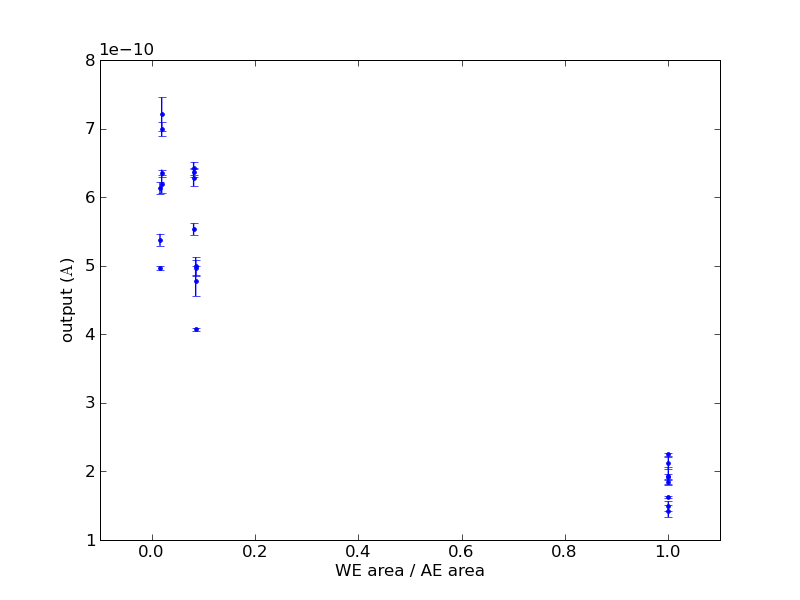
\includegraphics[width=0.7\linewidth]{figures/area_ratio_v_output.png}
	\caption{WE area / AE area vs. Output}
	\label{area_ratio_v_output}
\end{figure}

\subsection{Working Electrode Perimeter over Area vs. Output Density}

This hypothesis is that the output current density is proportional to the WE perimeter divided by the WE area. Figure \ref{perim_area_v_density} shows the tests and a linear-fit curve. We can see a correlation, indicating that most of the electron transfer happens near the edge of the electrode.

\begin{figure}
	\centering
	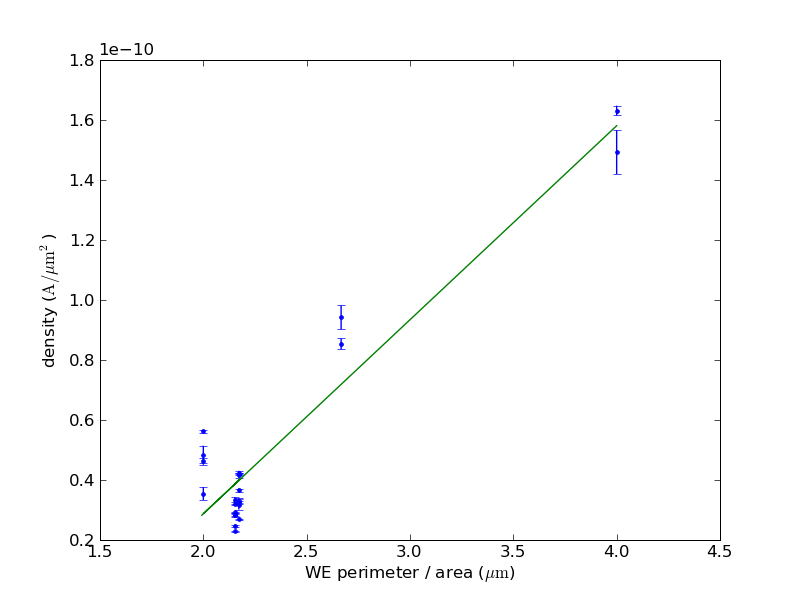
\includegraphics[width=0.7\linewidth]{figures/perim_area_v_density.png}
	\caption{WE perimeter / area vs. Density}
	\label{perim_area_v_density}
\end{figure}

\subsection{Distance from Working to Auxiliary Electrode}

This hypothesis is that the output current density is proportional to the distance from the WE to the AE. Figure \ref{distance_v_density} shows the tests. The vertical column below 5 microns contains all ``2 auxiliary'' sensor configurations, which are only 3-electrode systems. It is clear that the data are inconclusive, and that distance plays an unimportant part for most electrodes.

\begin{figure}
	\centering
	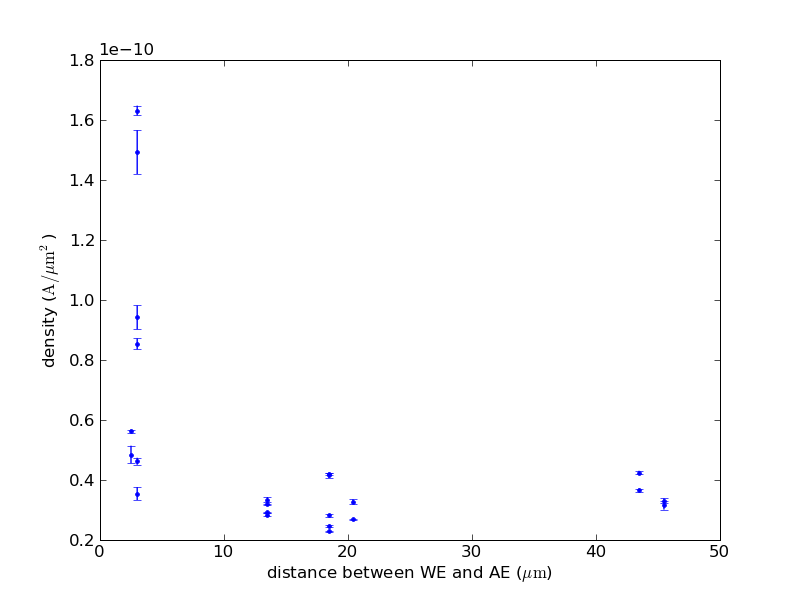
\includegraphics[width=0.7\linewidth]{figures/distance_v_density.png}
	\caption{Distance from WE to AE vs. Density}
	\label{distance_v_density}
\end{figure}

\section{Limit of Detection Results}

Sensor 17 (Table \ref{limit 17}) was able to detect down to about 3$\mu$M with a linear fit of $A = 1.88996 * 10^{-6} * M - 2.36855 * 10^{-12}$, where $A$ is the resulting current in amperes and $M$ is the concentration molarity. Sensor 8 (Table \ref{limit 8}) was able to detect down to about 10$\mu$M with a linear fit of $A = 8.29117 * 10^{-7} * M + 4.3417 * 10^{-11}$, where $A$ is the resulting current in amperes and $M$ is the concentration molarity. These are summarized in Figure \ref{limit figure}.

\begin{table}
	\begin{tabular}{ll}
		Concentration (M) & Peak value \\
		\hline
		0.0003 & 5.609E-10 \\
		0.0003 & 5.591E-10 \\
		0.0001 & 1.988E-10 \\
		0.0001 & 2.082E-10 \\
		0.000033 & 5.701E-11 \\
		0.000033 & 4.788E-11 \\
		0.000011 & 1.306E-11 \\
		0.000011 & 1.439E-11 \\
	\end{tabular}
	\caption[Detection limit results for sensor 17]{Detection limit results for sensor 17 sorted by decreasing concentration}
	\label{limit 17}
\end{table}

\begin{table}
	\begin{tabular}{ll}
		Concentration (M) & Peak value \\
		\hline
		0.0003 & 2.926E-10 \\
		0.0003 & 2.663E-10 \\
		0.0001 & 1.786E-10 \\
		0.0001 & 1.753E-10 \\
		0.000033 & 3.276E-11 \\
		0.000033 & 3.296E-11 \\
	\end{tabular}
	\caption[Detection limit results for sensor 8]{Detection limit results for sensor 8 sorted by decreasing concentration}
	\label{limit 8}
\end{table}

\begin{figure}
	\centering
	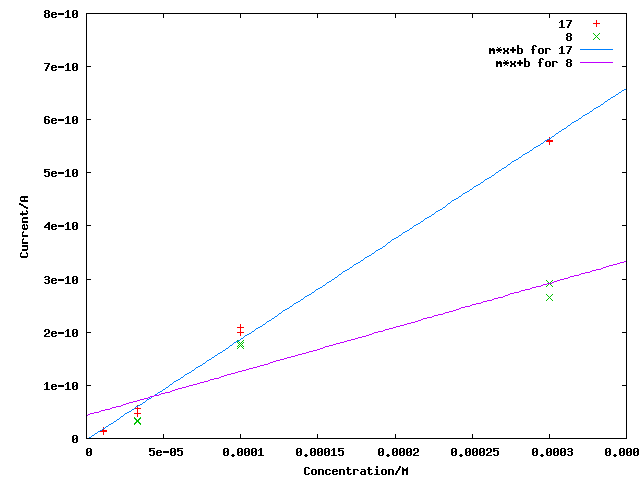
\includegraphics[width=0.7\linewidth]{figures/limit.png}
	\caption{Detection limits}
	\label{limit figure}
\end{figure}
